\section{Experiments}\label{sec:experiment}
We experimentally evaluated the performance and quality of our methodology (heuristic algorithm in \cref{subsec:heuristics}), and compared it against the exhaustive approach in~\cref{sec:nphard} {\color{OurColor}and our baseline modeling solutions in the state of the art in~\cref{subsec:experiments_infrastructure}.} In the following,
\cref{subsec:experiments_infrastructure} presents the simulator and experimental settings used in our experiments;
\cref{subsec:experiments_performance} analyses the performance of our solution in terms of execution time; \cref{subsec:experiments_quality} discusses the quality of the best pipeline instance generated by our solution according to the metrics $M_J$ and $M_{JSD}$ in \cref{subsec:metrics}.

\subsection{Testing Infrastructure and Experimental Settings}\label{subsec:experiments_infrastructure}
Our testing infrastructure is a Swift-based simulator of a service-based ecosystem, including service execution, selection, and composition.
The simulator first defines the pipeline template as a sequence of vertices, with $l$ the length of the pipeline template, and defines the size \windowsize\ of the sliding window, such that \windowsize$\leq$$l$. We recall that alternative vertices are modeled in different pipeline templates, while parallel vertices are not considered in our experiments since they only add a fixed execution time that is negligible and does not affect the performance and quality of our solution. Each vertex is associated with a (set of) policy that applies a filtering transformation that removes a given percentage of data.


      The simulator then starts the instantiation process. At each step $i$, it selects the subset \{\vi{i},$\ldots$,$v_{\windowsize+i-1}$\} of vertices with their corresponding candidate services, and generates all possible service combinations. The simulator calculates quality $Q$ for all combinations and instantiates \vi{i} with service \sii{i} from the optimal combination with maximum $Q$. The window is shifted by 1 (i.e., $i$=$i$+1), and the instantiation process restarts. When the sliding window reaches the end of the pipeline template, that is, $v_{\windowsize+i-1}$$=$$\vi{l}$, the simulator computes the optimal service combination and instantiates the remaining vertices with the corresponding services. \cref{fig:execution_example} shows an example of a simulator execution with $i$$=$2 and \windowsize$=$3. Subset \{\vi{2},\vi{3},\vi{4}\} is selected, all combinations generated, and corresponding quality $Q$ calculated. Optimal service combination \{\sii{11},\sii{22},\sii{31}\} is retrieved and \vii{2} in the pipeline instance instantiated with \sii{11}.

    \begin{figure}[!t]
      \centering
      \resizebox{0.7\columnwidth}{!}{%
        \begin{tikzpicture}[framed]

          \node[draw, circle, fill=gray!40,minimum width=0.7cm] (v1) at (1,5.2) {$\vi{1}$};
          \node[draw, circle, fill=gray!40,minimum width=0.7cm] (v2) at (3,5.2) {$\vi{2}$};
          \node[draw, circle, fill=gray!40,minimum width=0.7cm] (v3) at (5,5.2) {$\vi{3}$};
          \node[draw, circle, fill=gray!40,minimum width=0.7cm] (v4) at (7,5.2) {$\vi{4}$};
          \node[draw, circle, fill=gray!40,minimum width=0.7cm] (v5) at (9,5.2) {$\vi{5}$};
          \node[above, shift=({0,0.5}),  ] at (v3.north)  {Sliding Window};

          \node[draw, rectangle,fill=red!20] (s1) at (1,3.4) {$\sii{1}$};
          \node[draw, rectangle, fill=green!20] (s2) at (1,1.7) {$\sii{2}$};
          \node[draw, rectangle, fill=red!20] (s3) at (1,0) {$\sii{3}$};

          \node[draw, rectangle,thick] (s11) at (3,3.4) {$\sii{11}$};
          \node[draw, rectangle,opacity=.6] (s12) at (3,1.7) {$\sii{12}$};
          \node[draw, rectangle,opacity=.6] (s13) at (3,0) {$\sii{13}$};

          \node[draw, rectangle,opacity=.6] (s21) at (5,3.4) {$\sii{21}$};
          \node[draw, rectangle,thick] (s22) at (5,1.7) {$\sii{22}$};
          \node[draw, rectangle,opacity=.6] (s23) at (5,0) {$\sii{23}$};

          \node[draw, rectangle, thick] (s31) at (7,3.4) {$\sii{31}$};
          \node[draw, rectangle,opacity=.6] (s32) at (7,1.7) {$\sii{32}$};
          \node[draw, rectangle,opacity=.6] (s33) at (7,0) {$\sii{33}$};

          \node[draw, rectangle] (s41) at (9,3.4) {$\sii{41}$};
          \node[draw, rectangle] (s42) at (9,1.7) {$\sii{42}$};
          \node[draw, rectangle] (s43) at (9,0) {$\sii{43}$};

          \draw[->,line width= 1.2pt] (s2) -- (s11);
          \draw[->,dashdotted] (s2) -- (s12);
          \draw[->,dashdotted] (s2) -- (s13);

          \draw[->,line width= 1pt] (s11) -- (s22);

          \draw[->,dashdotted] (s11) -- (s21);
          \draw[->,dashdotted] (s11) -- (s23);

          \draw[->,dashdotted] (s12) -- (s21);
          \draw[->,dashdotted] (s12) -- (s22);
          \draw[->,dashdotted] (s12) -- (s23);

          \draw[->,dashdotted] (s13) -- (s21);
          \draw[->,dashdotted] (s13) -- (s22);
          \draw[->,dashdotted] (s13) -- (s23);

          \draw[->,dashdotted] (s21) -- (s31);
          \draw[->,dashdotted] (s21) -- (s32);
          \draw[->,dashdotted] (s21) -- (s33);

          \draw[->,line width=1pt] (s22) -- (s31);
          \draw[->,dashdotted] (s22) -- (s32);
          \draw[->,dashdotted] (s22) -- (s33);

          \draw[->,dashdotted] (s23) -- (s31);
          \draw[->,dashdotted] (s23) -- (s32);
          \draw[->,dashdotted] (s23) -- (s33);

          \draw[->] (v1) -- (v2);
          \draw[->] (v2) -- (v3);
          \draw[->] (v3) -- (v4);
          \draw[->] (v4) -- (v5);

          \begin{scope}[on background layer]
            \draw[thick, dashed, fill=red!10, opacity=0.5]
            ([shift={(-0.5,0.5)}]s11.north west) rectangle ([shift={(0.5,-0.5)}]s33.south east);

          \end{scope}
          \begin{scope}[on background layer]
            \draw[thick, dashed, fill=red!10, opacity=0.5]
            ([shift={(-0.5,0.5)}]v2.north west) rectangle ([shift={(0.5,-0.5)}]v4.south east);

          \end{scope}

        \end{tikzpicture}
      }
      \caption{Execution example of the sliding window heuristic using v=5, s=3, \windowsize=3 at i=1 step.}
      \label{fig:execution_example}
    \end{figure}

    The simulator defines dependencies between filtering transformations made by candidate services at consecutive vertices of the pipeline template.
    To this aim, it assigns a dependency rate to each service \si{i} modeling the amount of the filtering transformation done at \si{i} that overlaps the one at \si{i-1}.
    For example, let us consider the pairs of services (\si{11},\si{21}) and (\si{11},\si{22}) with the following configurations: \emph{i)} service \si{11} introduces a filtering transformation that removes the 20\% of the dataset, \emph{ii)} service \si{21} introduces a filtering transformation that removes 10\% of the dataset and has dependency rate equal to 1, meaning that the filtering transformation made by \si{21} completely overlaps the one made by \si{11}, \emph{iii)} service \si{22} introduces a filtering transformation that removes 5\% of the dataset and has dependency rate equal to 0.5, meaning that the filtering transformation made by \si{22} overlaps half of the one made by \si{11}. Jaccard Metric $M_{J_{21}}$$=$0.8 at service \si{21}; $M_{J_{22}}$$=$0.775 at \si{22}, showing how dependencies can affect the pipeline quality and, in turn, the instantiation process.


    Our simulator also supports the comparison of the performance and quality of our sliding-window heuristic with \emph{i)} a baseline modeling solutions in the state of the art and \emph{ii)} the exhaustive approach (i.e., the theoretical optimum). We modeled our baseline as a greedy approach that, for each node of the service pipeline, selects the best service that maximizes the data quality, while addressing data protection requirements in annotation $\myLambda$. The reason is that, to the best of our knowledge, existing (industry) solutions and standards do not support service-based data pipelines and are therefore unable to instantiate the service pipeline according to the pipeline structure and service dependencies. We therefore defined our baseline as the sliding window heuristic configured with window size $|$w$|$=1.
    We implemented the exhaustive approach calculating the theoretical optimum as the sliding window heuristic configured with window size $|$w$|$=$l$, to illustrate the potential efficiency of our heuristics within realistic computational limits.



    Our experiments have been run on a virtual machine equipped with an Intel(R) Xeon(R) CPU E5-2620 v4 @ 2.10GHz CPU and 32GB RAM. Each experiment was repeated 10 times and the results averaged to improve the reliability of findings.



    \begin{table}[!t]
      \caption{Experimental Parameters}
      \label{tab:parameters}
      \centering
      {\color{OurColor2}
        \begin{tabular}{l|l}
          \textbf{Parameter}                  & \textbf{Values}  \\
          \hline
          Window Size (\textbar{}w\textbar{}) & 2, 3, 4, 5, 6, 7 \\
          Filtering Configuration                & wide, average\\
          Number of Candidate Services        & 2, 3, 4, 5, 6, 7 \\
          Number of Pipeline Vertices            & 2, 3, 4, 5, 6, 7 \\
          Metrics                             & quantitative ($M_J$), qualitative ($M_{JSD}$) \\
        \end{tabular}
      }
    \end{table}
  {\color{OurColor2}
  \cref{tab:parameters} summarizes the parameters and corresponding values used in our experimental evaluation. The window size (\textbar{}w\textbar{}), ranging from 2 to 7, represents different configurations of our heuristic approach. The filtering configuration defines two representative filtering transformations: \textit{wide} removing a percentage of data in [0.2,1] and \textit{average} in [0.5,0.8]. Additionally, the number of candidate services and pipeline vertices, also varying from 2 to 7, models diverse configurations of service pipelines. The evaluation metrics include both quantitative ($M_J$) and qualitative ($M_{JSD}$) measures for the completeness dimension of quality, offering insights into the impact of data protection transformations on overall pipeline quality.
  }
    \subsection{Performance}\label{subsec:experiments_performance}
    We first measured the performance (execution time) of our exhaustive, baseline, and heuristic solutions by varying the number of vertices in the pipeline template from 2 to 7 and the number of services per vertex from 2 to 7. \cref{fig:time_window_perce_average} presents our results.
    The exhaustive approach can provide the optimal solution for all configurations, but its execution time grows exponentially with the number of vertices and services, making it impractical for large instances. For \windowsize\ from 1 to 3 (step 1), we observed a substantial reduction in execution time, with the heuristic always able to produce an instance in less than $\approx2.7\times10^5ms$ . The worst heuristic performance (7 vertices, 7 services, \windowsize=6) is $\approx3.8\times10^7ms$, one order of magnitude lower than the best exhaustive performance (7 vertices, 7 services, \windowsize=7) $\approx1.35\times10^8ms$. {\color{OurColor} As expected, the baseline (i.e., our heuristic with \windowsize$=$1) shows the best performance in all settings.}
    \begin{figure}[!t]
      \centering
      \begin{subfigure}{0.45\textwidth}
        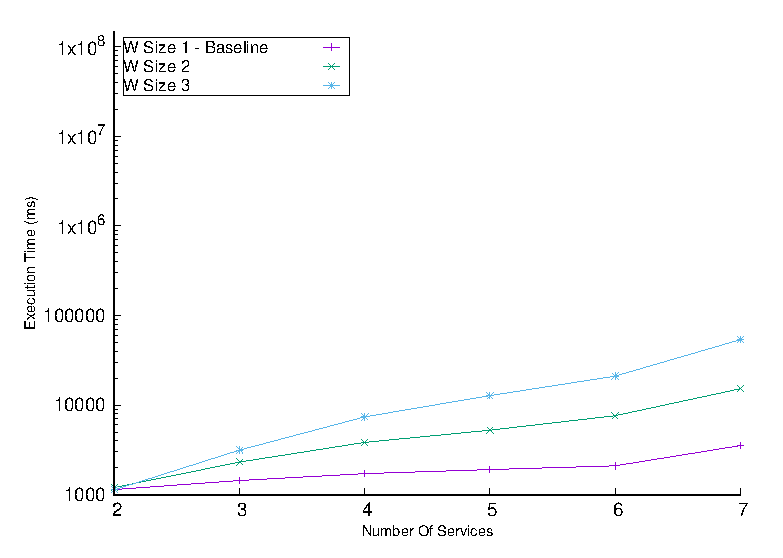
\includegraphics[width=\textwidth]{Images/graphs/window_time_performance_qualitative_n7_s7_50_80_n3}
        \caption{3 vertices}
        \label{fig:time_window_perce_wide_3n}
      \end{subfigure}
      \hfill
      \begin{subfigure}{0.45\textwidth}
        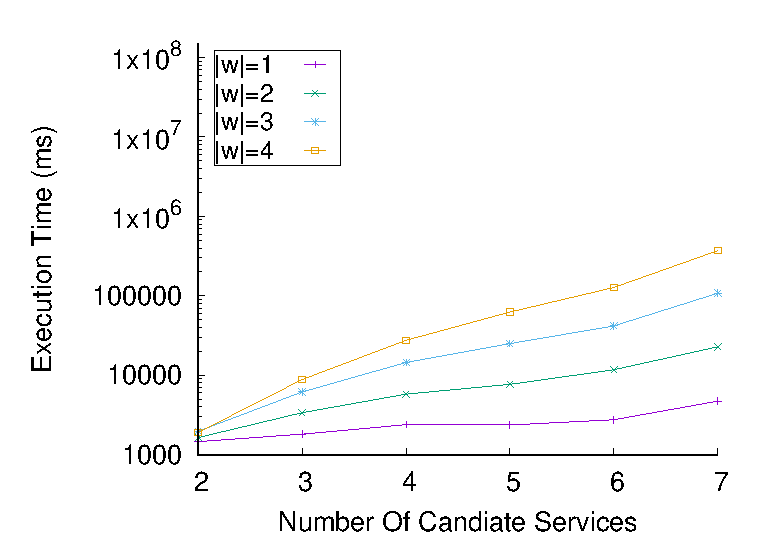
\includegraphics[width=\textwidth]{Images/graphs/window_time_performance_qualitative_n7_s7_50_80_n4}
        \caption{4 vertices}
        \label{fig:time_window_perce_wide_4n}
      \end{subfigure}
      \hfill
      \begin{subfigure}{0.45\textwidth}
        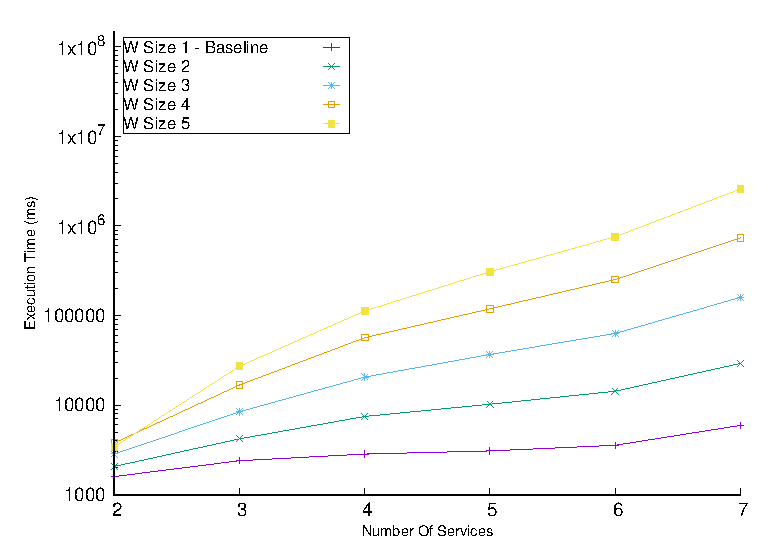
\includegraphics[width=\textwidth]{Images/graphs/window_time_performance_qualitative_n7_s7_50_80_n5}
        \caption{5 vertices}
        \label{fig:time_window_perce_wide_5n}
      \end{subfigure}
      \hfill
      \begin{subfigure}{0.45\textwidth}
        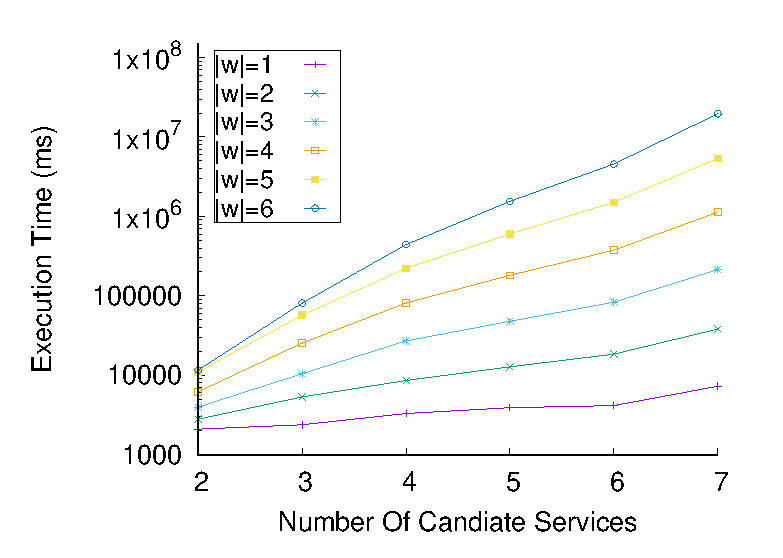
\includegraphics[width=\textwidth]{Images/graphs/window_time_performance_qualitative_n7_s7_50_80_n6}
        \caption{6 vertices}
        \label{fig:time_window_perce_wide_6n}
      \end{subfigure}
      \begin{subfigure}{0.45\textwidth}
        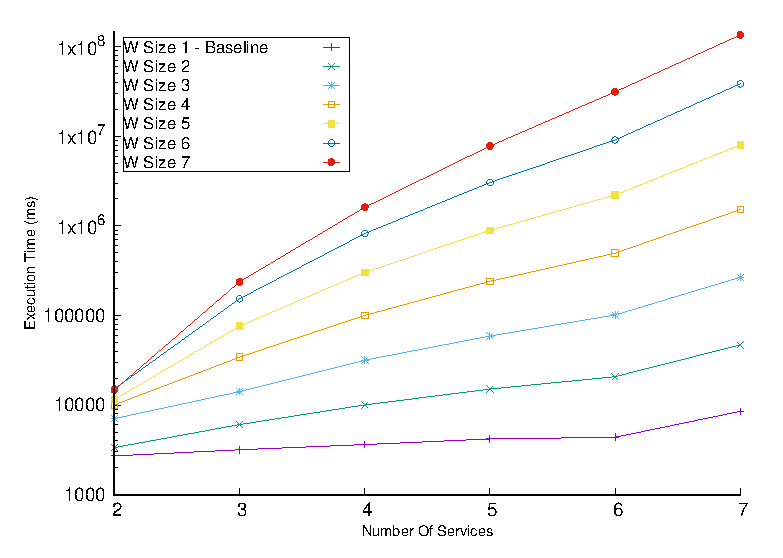
\includegraphics[width=\textwidth]{Images/graphs/window_time_performance_qualitative_n7_s7_50_80_n7}
        \caption{7 vertices}
        \label{fig:time_window_perce_wide_7n}
      \end{subfigure}
      \caption{{\color{OurColor2}Evaluation of Performance Using the \emph{Qualitative} Metric in a \average Configuration}}
      \label{fig:time_window_perce_average}
    \end{figure}

    \subsection{Quality}\label{subsec:experiments_quality}
    We evaluated the quality of our heuristic algorithm with different \windowsize\ comparing its results with the baseline and, where possible, with the optimal solution retrieved by executing the exhaustive approach.
    The quality $Q$ of the heuristic has been normalized between 0 and 1 by dividing it by the quality $Q^*$ retrieved by the exhaustive approach.

    We run our experiments varying: \emph{i)} the length $l$ of the pipeline template in [3,7], that is, the depth of the pipeline template as the number of vertices composed in a sequence, \emph{ii)} the window size \windowsize\ in [1,$l$], and \emph{iii)} the number of candidate services for each vertex in the pipeline template in [2, 7]. Each vertex is associated with a (set of) policy that applies a filtering transformation that either removes a percentage of data in $[0.5,0.8]$ (\average) or in $[0.2,1]$ (\wide).

      {\color{OurColor2}\cref{fig:quality_window_perce} presents}  our quality results using metric $M_J$ in \cref{subsec:metrics} for settings \wide and \average.
    In general, we observe that the quality of our heuristic approach increases as the window size increases, providing a quality comparable to the exhaustive approach when the window size \windowsize\ approaches the length $l$ of the pipeline template.

    When considering setting \wide, the baseline (\windowsize=1) provides good results on average (0.71, 0.90), while showing substantial quality oscillations in specific runs: between 0.882 and 0.970 for 3 vertices, 0.810 and 0.942 for 4 vertices, 0.580 and 0.853 for 5 vertices, 0.682 and 0.943 for 6 vertices, 0.596 and 0.821 for 7 vertices. This same trend emerges when the window size is $<$$l$/2, while it starts approaching the optimum when the window size is $\geq$$l$/2. For instance, when \windowsize=$l$-1, the quality varies between 0.957 and 1.0 for 3 vertices, 0.982 and 1.0 for 4 vertices, 0.986 and 0.998 for 5 vertices, 0.977 and 1.0 for 6 vertices, 0.996 and 1.0 for 7 vertices.

    \begin{figure}[H]
      \centering
      \begin{adjustbox}{minipage=\linewidth,scale=0.75}
        \begin{subfigure}{0.45\textwidth}
          \begin{subfigure}{\textwidth}
            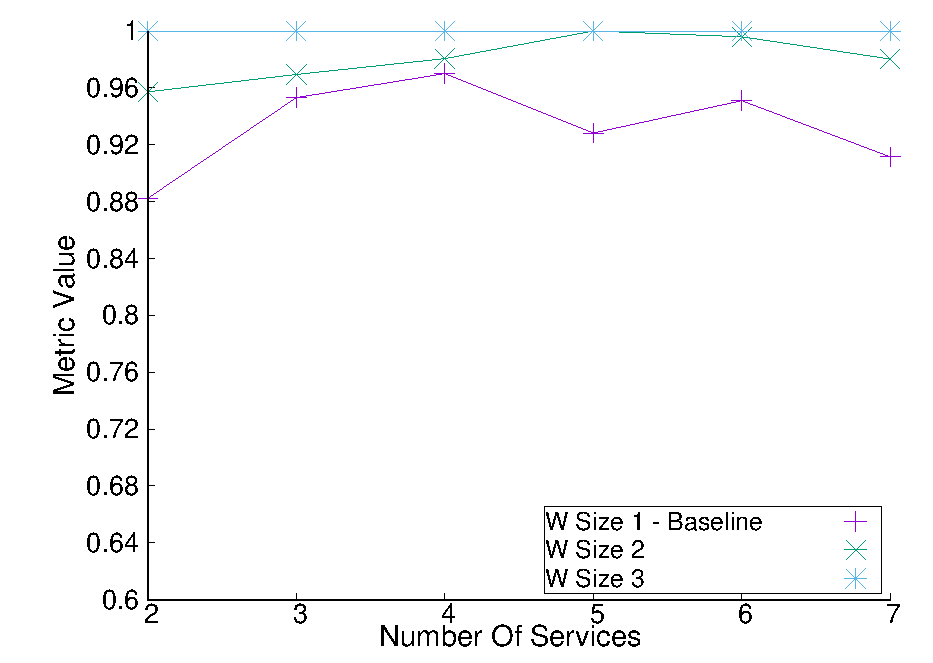
\includegraphics[width=\textwidth]{Images/graphs/window_quality_performance_diff_perce_n7_s7_20_100_n3}
            \caption{\wide 3 vertices}
            \label{fig:quality_window_wide_perce_n3}
          \end{subfigure}
          \begin{subfigure}{\textwidth}
            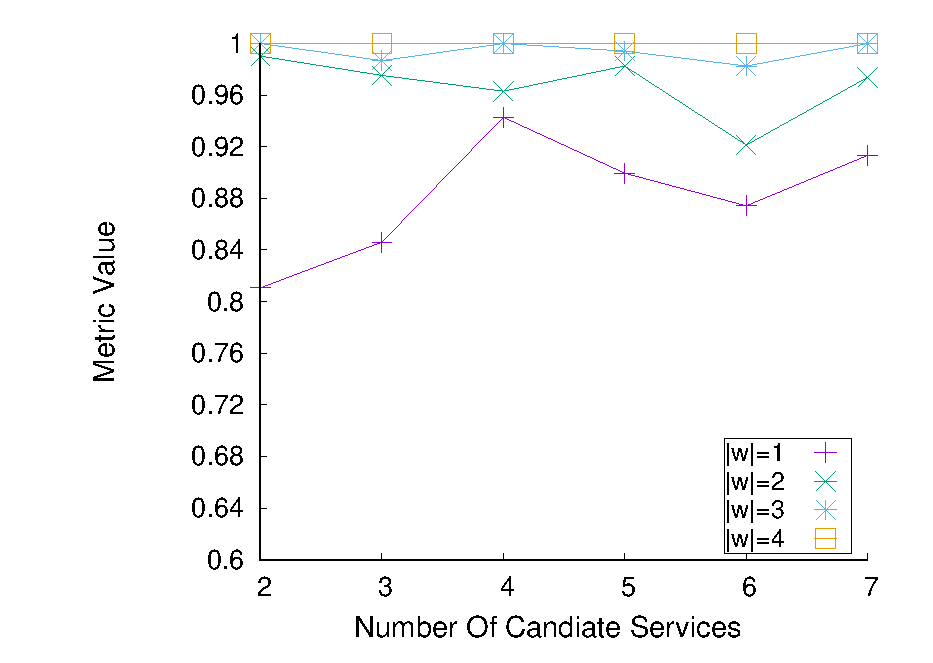
\includegraphics[width=\textwidth]{Images/graphs/window_quality_performance_diff_perce_n7_s7_20_100_n4}
            \caption{\wide 4 vertices}
            \label{fig:quality_window_wide_perce_n4}
          \end{subfigure}
          \begin{subfigure}{\textwidth}
            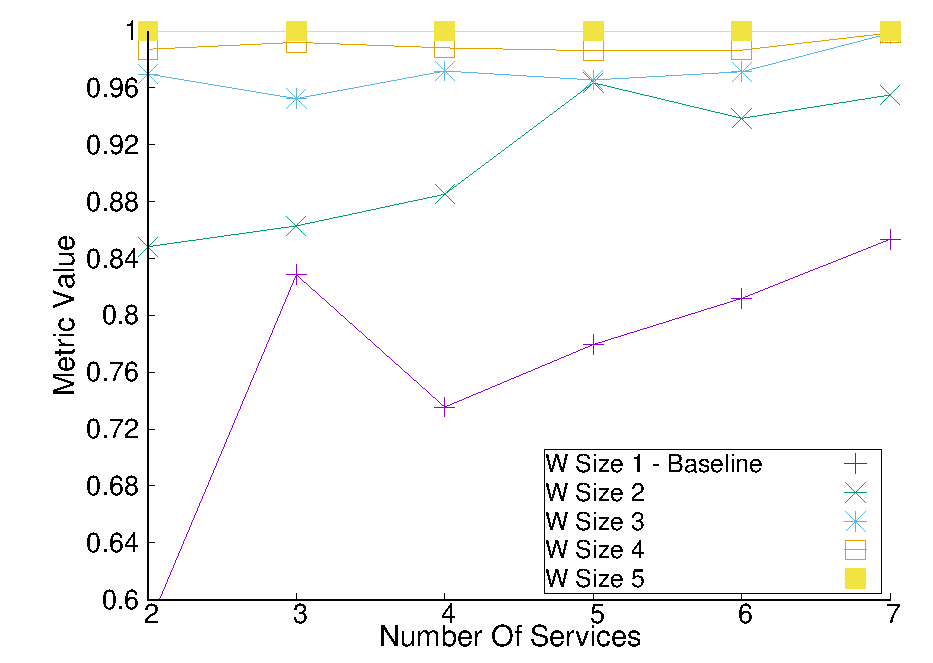
\includegraphics[width=\textwidth]{Images/graphs/window_quality_performance_diff_perce_n7_s7_20_100_n5}
            \caption{\wide 5 vertices}

            \label{fig:quality_window_wide_perce_n5}
          \end{subfigure}

          \begin{subfigure}{\textwidth}
            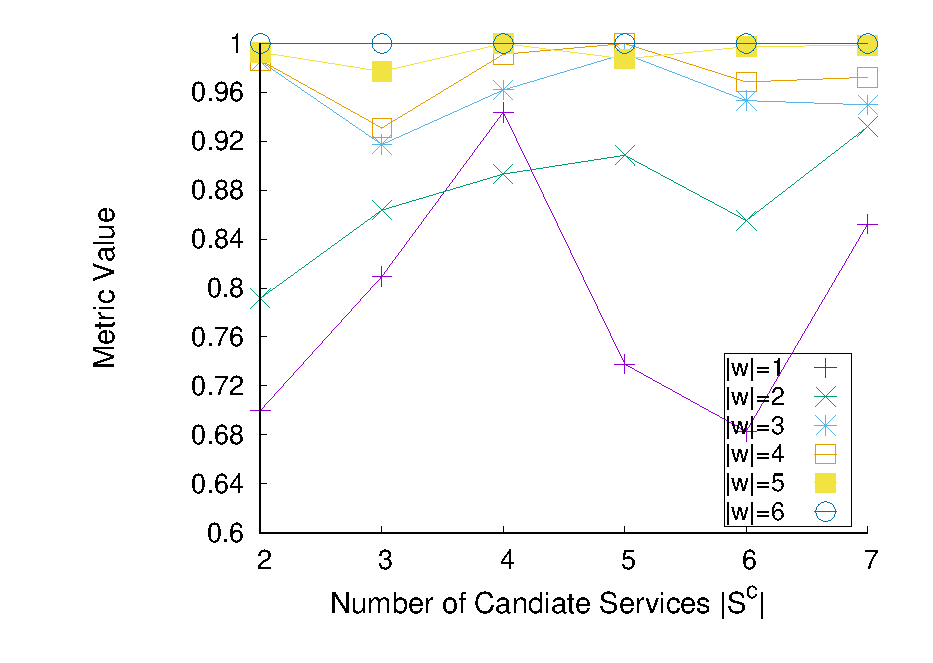
\includegraphics[width=\textwidth]{Images/graphs/window_quality_performance_diff_perce_n7_s7_20_100_n6}
            \caption{\wide 6 vertices}
            \label{fig:quality_window_wide_perce_n6}
          \end{subfigure}

          \begin{subfigure}{\textwidth}
            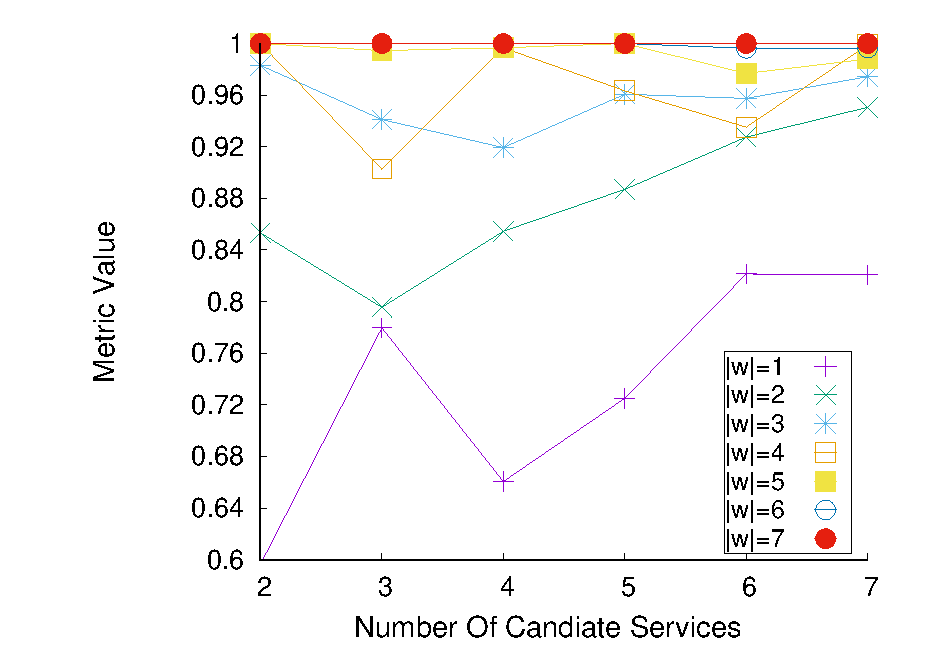
\includegraphics[width=\textwidth]{Images/graphs/window_quality_performance_diff_perce_n7_s7_20_100_n7}
            \caption{\wide 7 vertices}
            \label{fig:quality_window_wide_perce_n7}
          \end{subfigure}
        \end{subfigure}
        \begin{subfigure}{0.45\textwidth}
          \begin{subfigure}{\textwidth}
            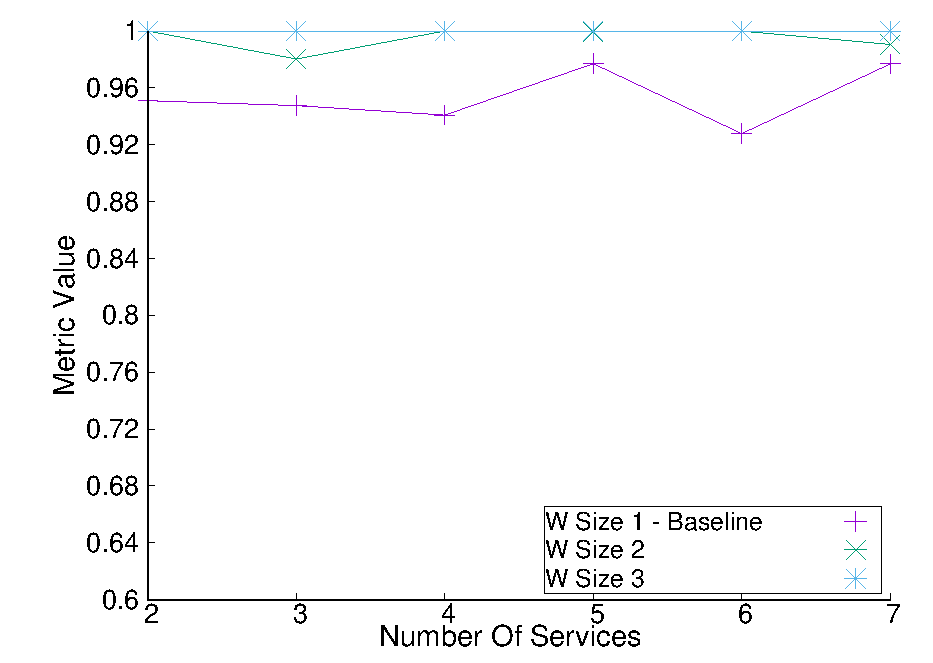
\includegraphics[width=\textwidth]{Images/graphs/window_quality_performance_diff_perce_n7_s7_50_89_n3}
            \caption{\average 3 vertices}

            \label{fig:quality_window_average_perce_n3}
          \end{subfigure}

          \begin{subfigure}{\textwidth}
            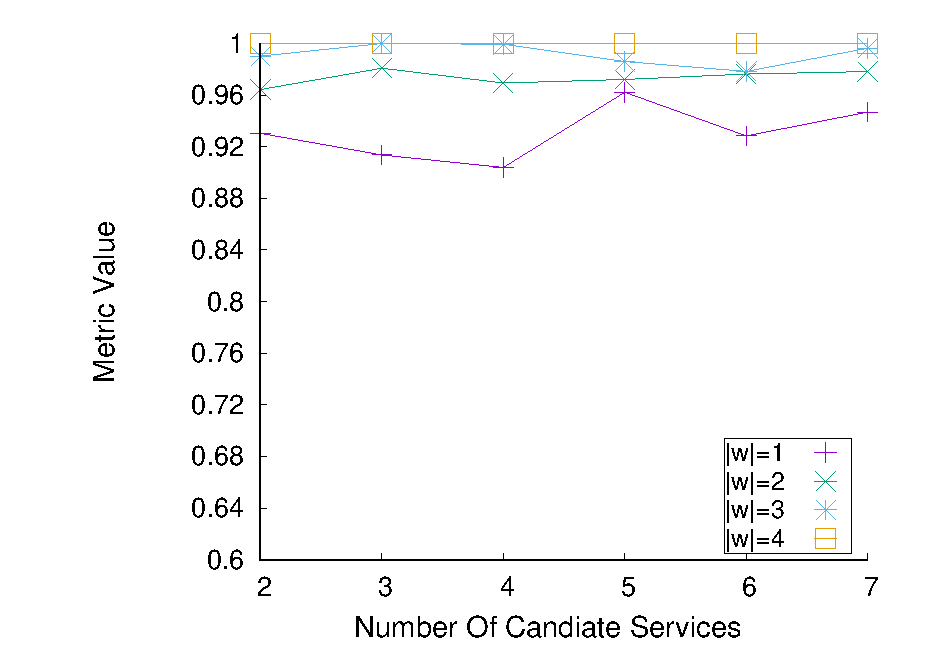
\includegraphics[width=\textwidth]{Images/graphs/window_quality_performance_diff_perce_n7_s7_50_89_n4}
            \caption{\average 4 vertices}

            \label{fig:quality_window_average_perce_n4}
          \end{subfigure}
          \begin{subfigure}{\textwidth}
            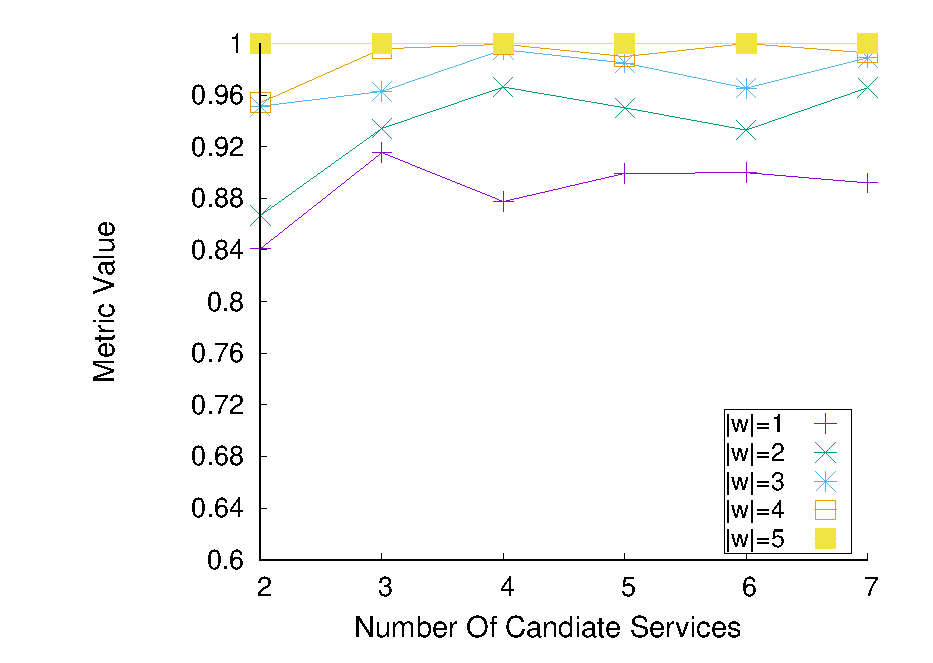
\includegraphics[width=\textwidth]{Images/graphs/window_quality_performance_diff_perce_n7_s7_50_89_n5}
            \caption{\average 5 vertices}
            \label{fig:quality_window_average_perce_n5}
          \end{subfigure}

          \begin{subfigure}{\textwidth}
            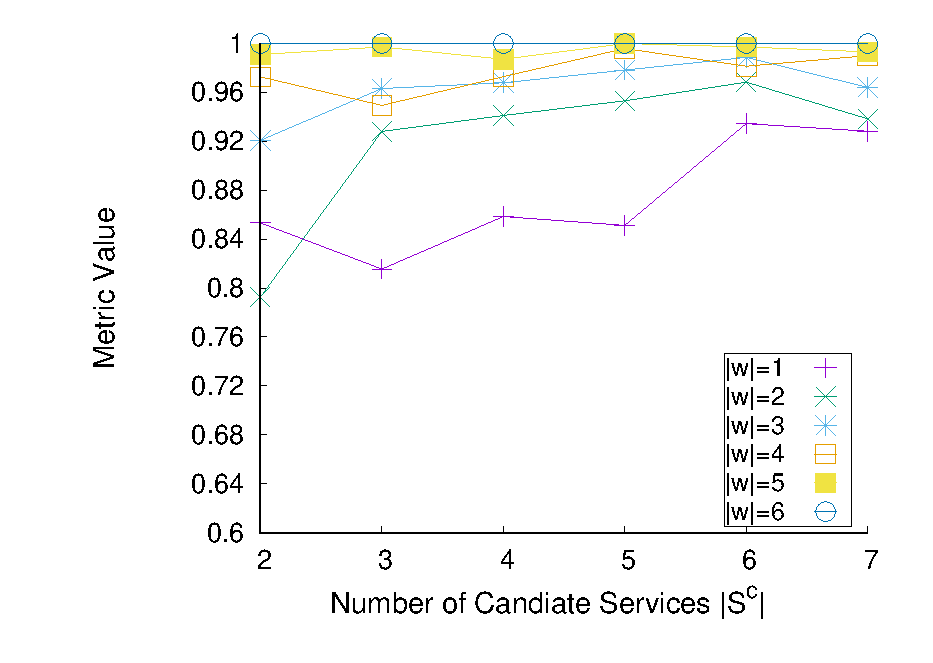
\includegraphics[width=\textwidth]{Images/graphs/window_quality_performance_diff_perce_n7_s7_50_89_n6}
            \caption{\average 6 vertices}
            \label{fig:quality_window_average_perce_n6}
          \end{subfigure}


          \begin{subfigure}{\textwidth}
            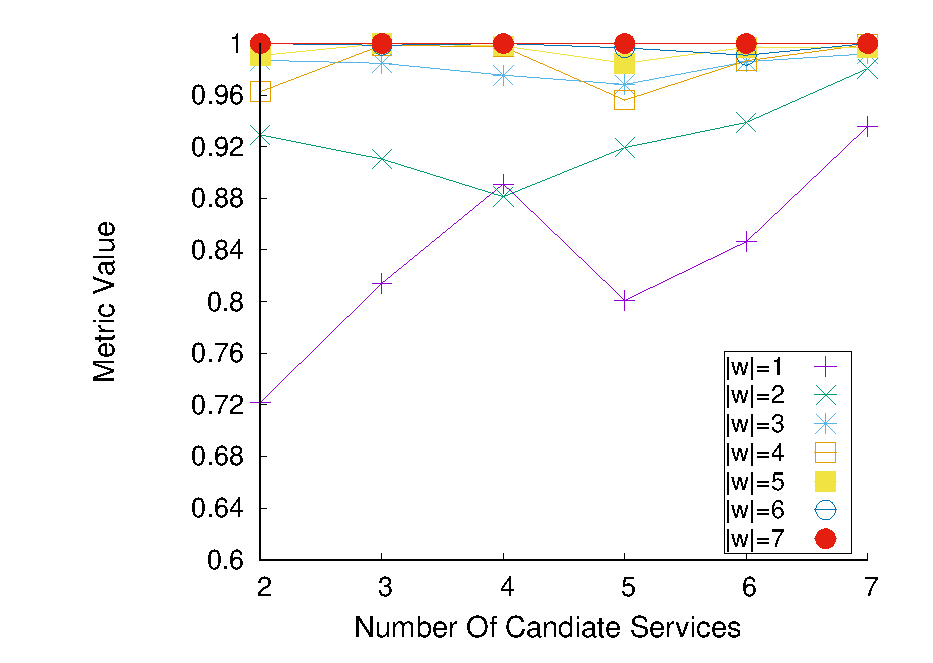
\includegraphics[width=\textwidth]{Images/graphs/window_quality_performance_diff_perce_n7_s7_50_89_n7}
            \caption{\average 7 vertices}
            \label{fig:quality_window_average_perce_n7}
          \end{subfigure}

        \end{subfigure}

        \caption{Evaluation of Quality Using the \emph{Quantitative} Metric in a \wide (\cref{fig:quality_window_wide_perce_n3,fig:quality_window_wide_perce_n4,fig:quality_window_wide_perce_n5,fig:quality_window_wide_perce_n6,fig:quality_window_wide_perce_n7}) and \average (\cref{fig:quality_window_average_perce_n3,fig:quality_window_average_perce_n4,fig:quality_window_average_perce_n5,fig:quality_window_average_perce_n6,fig:quality_window_average_perce_n7}) Configuration.}  \label{fig:quality_window_perce}
      \end{adjustbox}
    \end{figure}

    When considering setting \average, the heuristic algorithm still provides good results, limiting the quality oscillations observed for setting \wide\ and approaching the quality of the exhaustive also for lower window sizes. The baseline (\windowsize=1) provides good results on average (from 0.842 to 0.944), as well as in specific runs: between 0.927 and 0.978 for 3 vertices, 0.903 and 0.962 for 4 vertices, 0.840 and 0.915 for 5 vertices, 0.815 and 0.934 for 6 vertices, 0.721 and 0.935 for 7 vertices.
    When \windowsize=$l$-1, the quality varies between 0.980 and 1.0 for 3 vertices, 0.978 and 1.0 for 4 vertices, 0.954 and 1 for 5 vertices, 0.987 and 1.0 for 6 vertices, 0.990 and 1.0 for 7 vertices.

    \cref{fig:quality_window_qualitative} {\color{OurColor2}presents} our quality results using metric $M_{JSD}$ in \cref{subsec:metrics} for settings \wide and \average, respectively.

    When considering setting \wide, the baseline (\windowsize=1) provides good results on average (0.92, 0.97), limiting oscillations observed with metric $M_J$; for instance, the quality varies between 0.951 and 0.989 for 3 vertices, 0.941 and 0.988 for 4 vertices, 0.919 and 0.974 for 5 vertices, 0.911 and 0.971 for 6 vertices, 0.877 and 0.924 for 7 vertices.
    The worst quality results are obtained with the baseline, while the oscillations are negligible when the window size is $>$2. For instance, when \windowsize=$l$-2, the quality varies between, 0.982 and 0.996 for 4 vertices, 0.981 and 0.998 for 5 vertices, 0.988 and 1.0 for 6 vertices, 0.976 and 0.999 for 7 vertices. When \windowsize=$l$-1, the quality varies between  0.987 and  0.998 for 3 vertices, 0.993 and 1.0 for 4 vertices, 0.985 and 0.999 for 5 vertices, 0.997 and 1.0 for 6 vertices, 0.995 and 1.0  for 7 vertices.

\begin{figure}[H]
  \centering
  \begin{adjustbox}{minipage=\linewidth,scale=0.75}
    \begin{subfigure}{0.45\textwidth}
      \begin{subfigure}{\textwidth}
        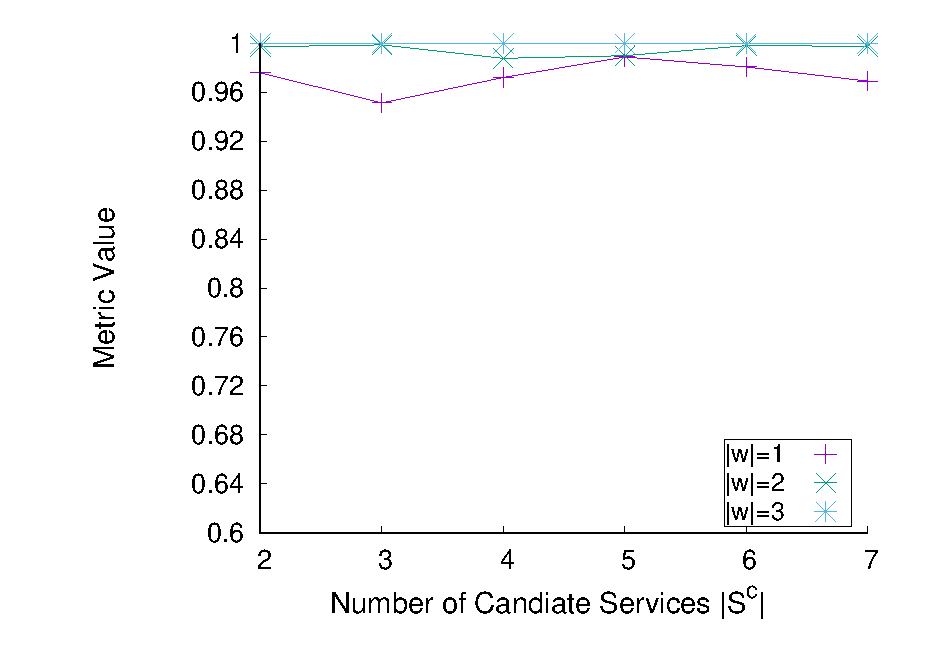
\includegraphics[width=\textwidth]{Images/graphs/window_quality_performance_diff_qual_n7_s7_20_100_n3}
        \caption{\wide 3 vertices}
        \label{fig:quality_window_wide_qualitative_n3}
      \end{subfigure}
      \begin{subfigure}{\textwidth}
        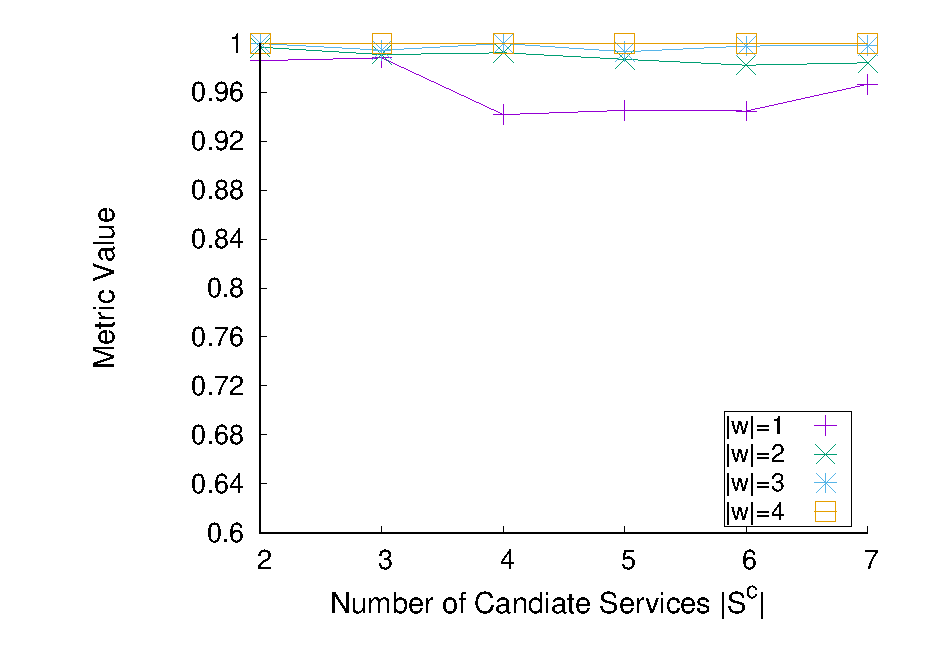
\includegraphics[width=\textwidth]{Images/graphs/window_quality_performance_diff_qual_n7_s7_20_100_n4}
        \caption{\wide 4 vertices}
        \label{fig:quality_window_wide_qualitative_n4}
      \end{subfigure}
      \begin{subfigure}{\textwidth}
        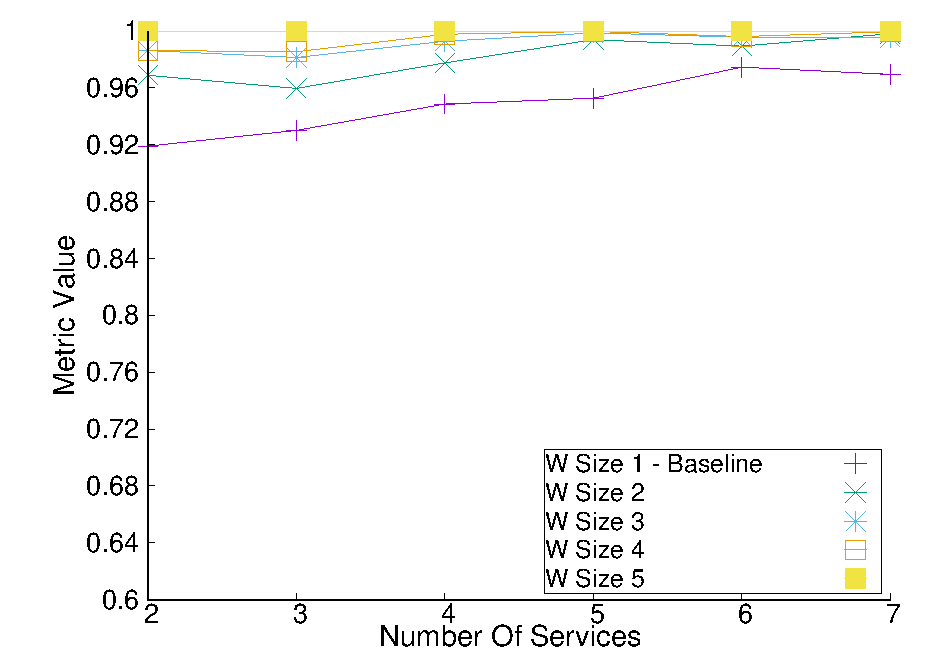
\includegraphics[width=\textwidth]{Images/graphs/window_quality_performance_diff_qual_n7_s7_20_100_n5}
        \caption{\wide 5 vertices}
        \label{fig:quality_window_wide_qualitative_n5}
      \end{subfigure}

      \begin{subfigure}{\textwidth}
        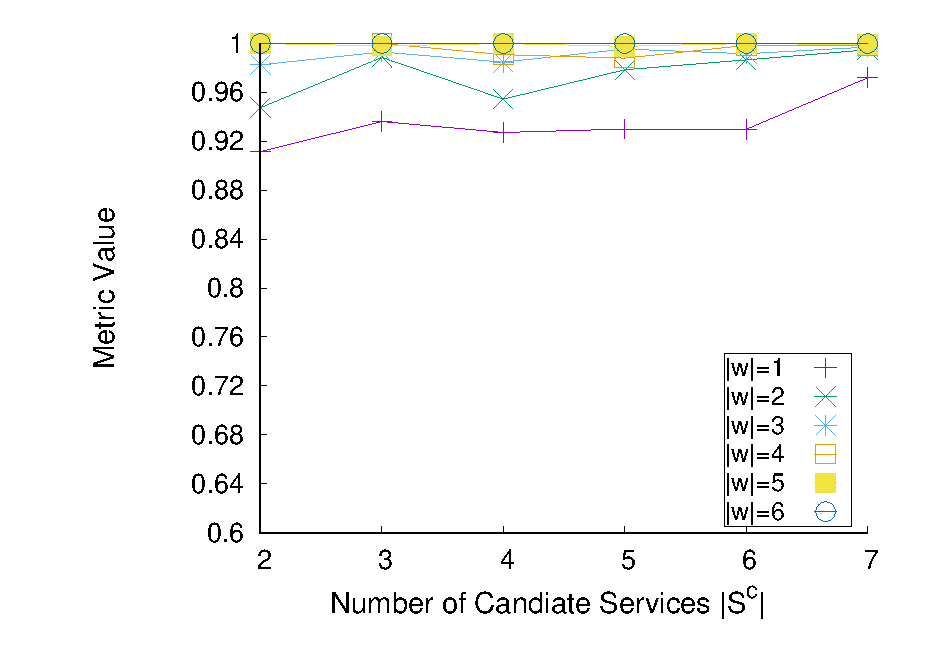
\includegraphics[width=\textwidth]{Images/graphs/window_quality_performance_diff_qual_n7_s7_20_100_n6}
        \caption{\wide 6 vertices}
        \label{fig:quality_window_wide_qualitative_n6}
      \end{subfigure}

      \begin{subfigure}{\textwidth}
        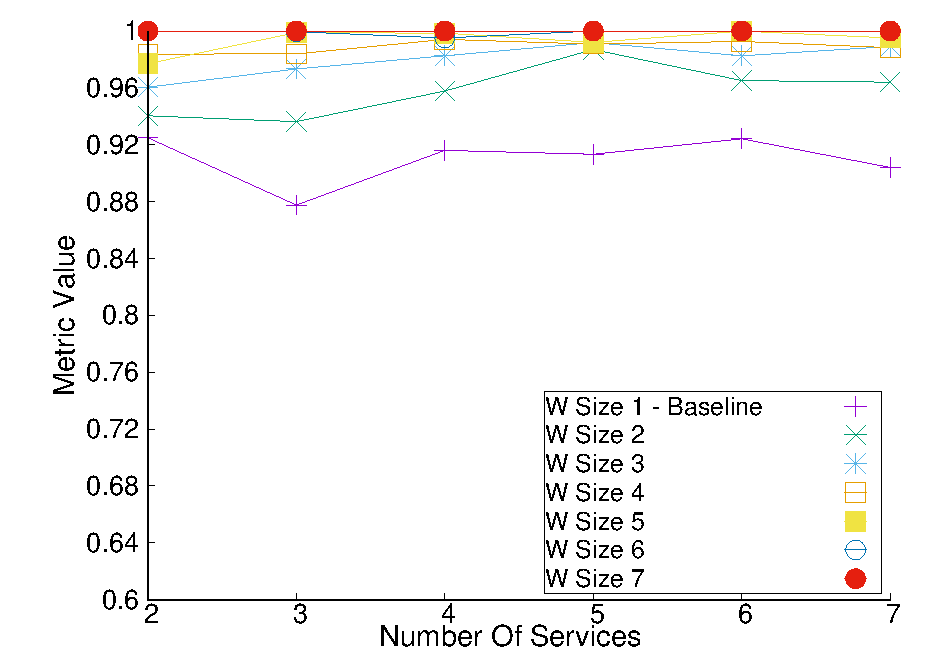
\includegraphics[width=\textwidth]{Images/graphs/window_quality_performance_diff_qual_n7_s7_20_100_n7}
        \caption{\wide 7 vertices}
        \label{fig:quality_window_wide_qualitative_n7}
      \end{subfigure}
    \end{subfigure}
    \begin{subfigure}{0.45\textwidth}
      \begin{subfigure}{\textwidth}
        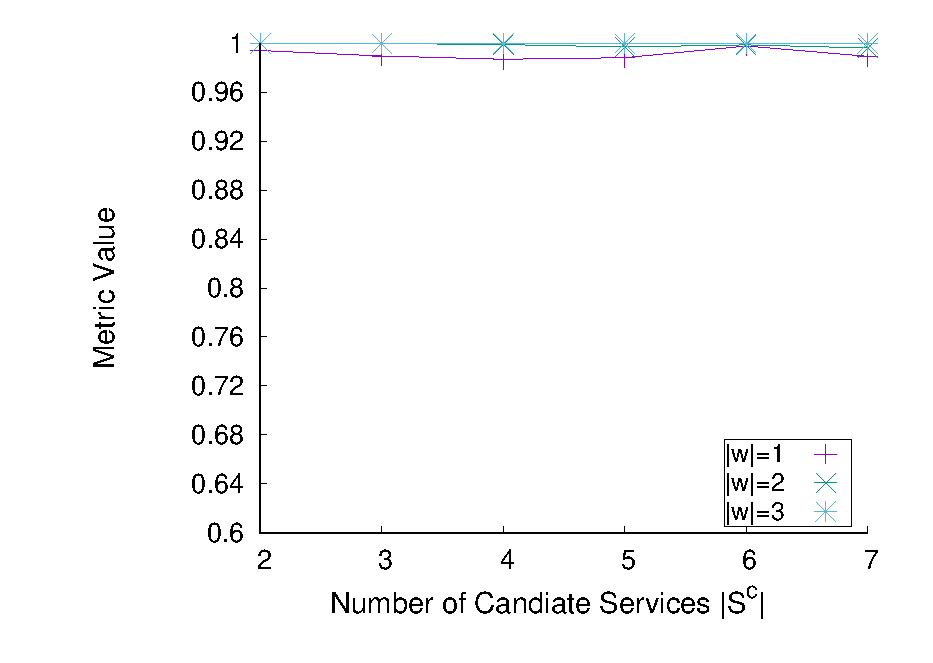
\includegraphics[width=\textwidth]{Images/graphs/window_quality_performance_diff_qual_n7_s7_50_80_n3}
        \caption{\average 3 vertices}
        \label{fig:quality_window_average_qualitative_n3}
      \end{subfigure}

      \begin{subfigure}{\textwidth}
        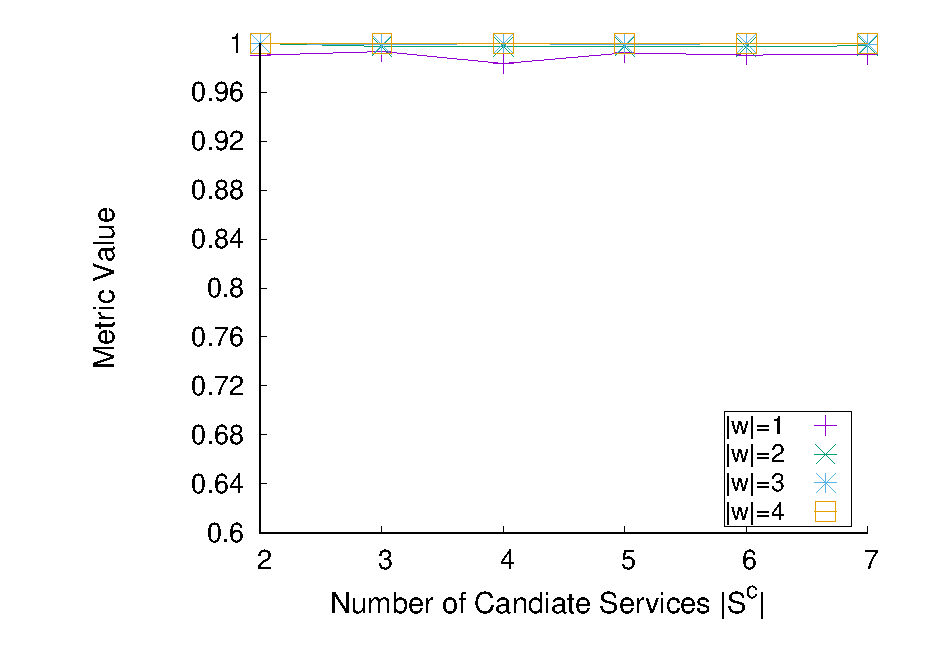
\includegraphics[width=\textwidth]{Images/graphs/window_quality_performance_diff_qual_n7_s7_50_80_n4}
        \caption{\average 4 vertices}
        \label{fig:quality_window_average_qualitative_n4}
      \end{subfigure}
      \begin{subfigure}{\textwidth}
        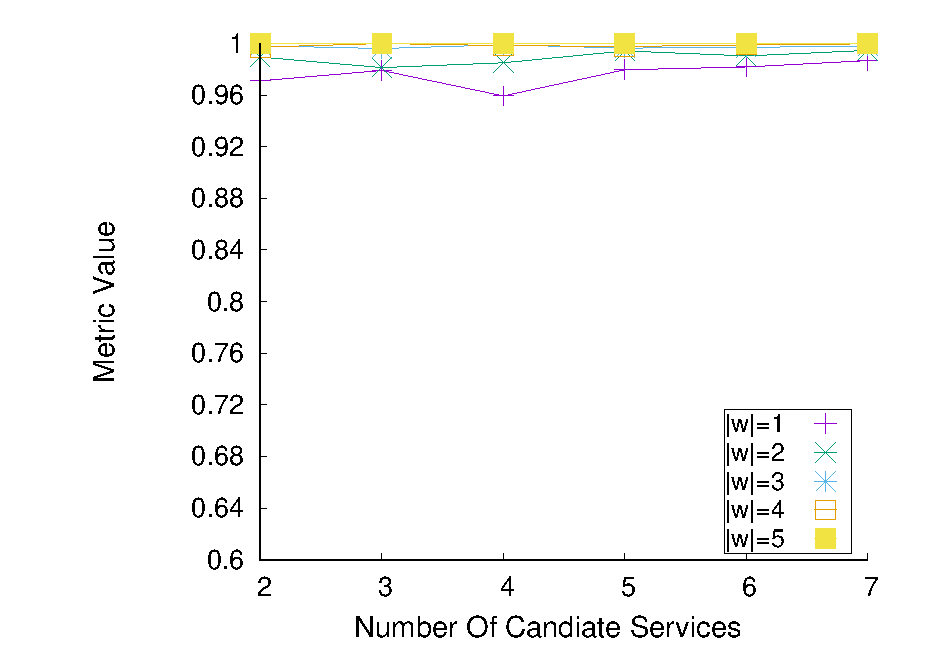
\includegraphics[width=\textwidth]{Images/graphs/window_quality_performance_diff_qual_n7_s7_50_80_n5}
        \caption{\average 5 vertices}
        \label{fig:quality_window_average_qualitative_n5}
      \end{subfigure}

      \begin{subfigure}{\textwidth}
        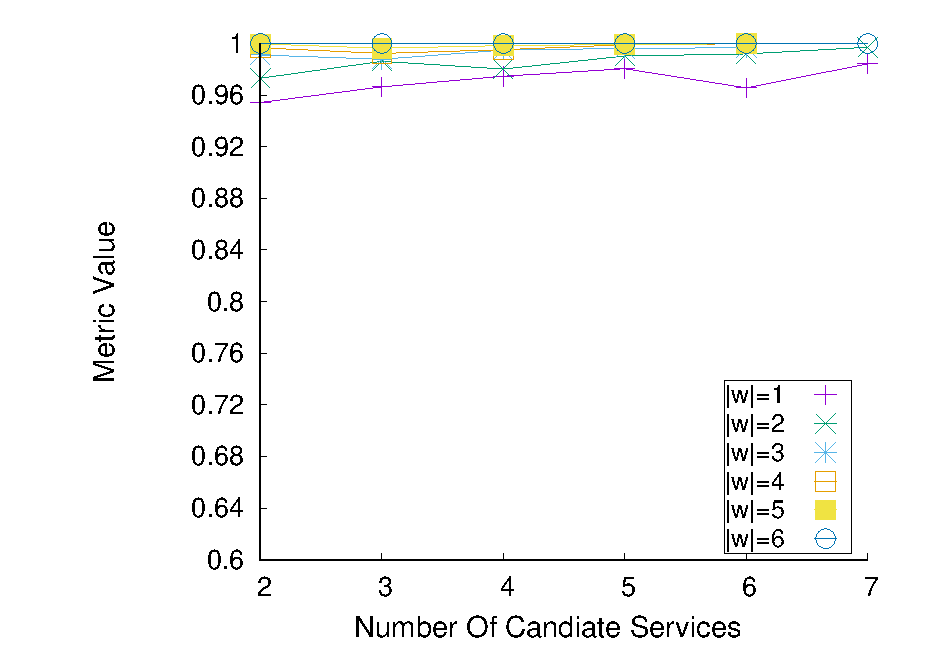
\includegraphics[width=\textwidth]{Images/graphs/window_quality_performance_diff_qual_n7_s7_50_80_n6}
        \caption{\average 6 vertices}
        \label{fig:quality_window_average_qualitative_n6}
      \end{subfigure}


      \begin{subfigure}{\textwidth}
        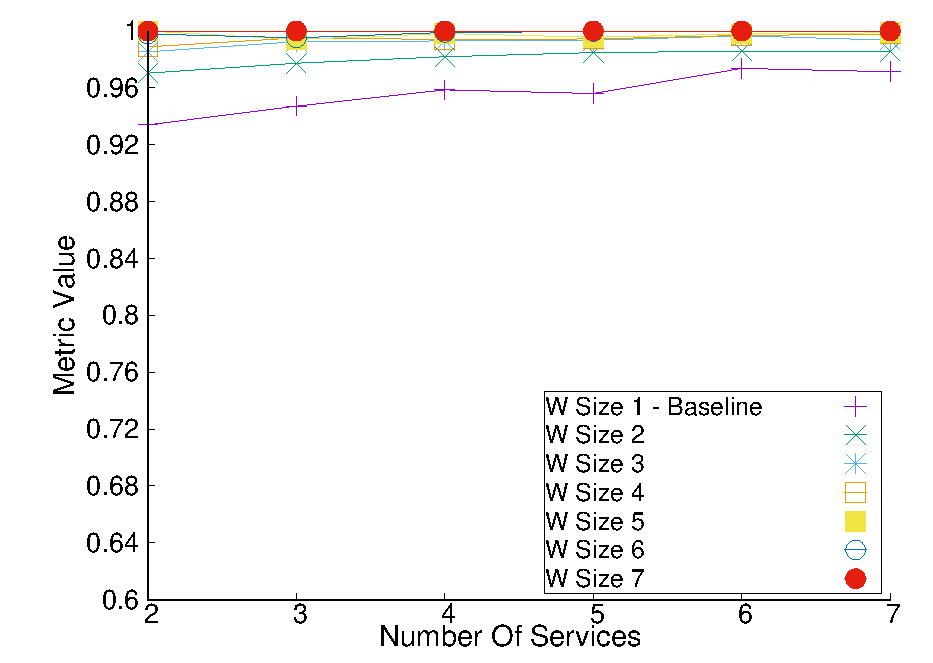
\includegraphics[width=\textwidth]{Images/graphs/window_quality_performance_diff_qual_n7_s7_50_80_n7}
        \caption{\average 7 vertices}
        \label{fig:quality_window_average_qualitative_n7}
      \end{subfigure}

    \end{subfigure}

    \caption{Evaluation of Quality Using the \emph{Qualitative} Metric in a \wide (\cref{fig:quality_window_wide_qualitative_n3,fig:quality_window_wide_qualitative_n4,fig:quality_window_wide_qualitative_n5,fig:quality_window_wide_qualitative_n6,fig:quality_window_wide_qualitative_n7}) and \average (\cref{fig:quality_window_average_qualitative_n3,fig:quality_window_average_qualitative_n4,fig:quality_window_average_qualitative_n5,fig:quality_window_average_qualitative_n6,fig:quality_window_average_qualitative_n7}) Configuration.}  \label{fig:quality_window_qualitative}
  \end{adjustbox}
\end{figure}

When considering setting \average, the baseline (\windowsize=1) provides results similar to setting \wide. On average, quality varies from 0.920 to 0.969, limiting oscillations; for instance, the quality varies between 0.951 and 0.989 for 3 vertices, 0.942 and 0.988 for 4 vertices, 0.919 and 0.975 for 5 vertices, 0.912 and 0.972 for 6 vertices, 0.878 and 0.925 for 7 vertices. The \average configuration provides even tighter quality oscillations than the \wide configuration. Notably, the poorest quality outcomes are observed with the baseline. Conversely, these oscillations become negligible when the window size exceeds 1 in configurations with three and four vertices, and when it exceeds 2 in configurations involving five, six, and seven vertices.  For instance, when \windowsize=3, the quality varies between  0.993 and 1 for 4 vertices, 0.981 and 0.998 for 5 vertices, 0.982 and 997 for 6 vertices, 0.960 and 0.991 for 7 vertices.


\subsection{Discussion}
The experimental results we obtained yield several valuable insights that merit further discussion. Three key observations emerged as follows.

\vspace{0.5em}

\noindent\textbf{Trade-off Between Execution Time and Quality.} As expected, the execution time improvement provided by our heuristic introduces a loss of quality with respect to the exhaustive approach. This loss causes an increase in the quality variance, especially when the window size (\windowsize) is small compared to the vertex count. A fine-grained tuning of heuristics is needed to balance computational efficiency and data quality.

\vspace{0.5em}

\noindent\textbf{Impact of Parameters on Quality.}
{\color{OurColor2}

Our experiments demonstrate that parameters in Table~3 can significantly influence the quality of the pipeline, with the number of service nodes and the window size emerging as key factors for both quality and performance.

Specifically, larger window sizes generally improve quality; however, there exists a balance point where the trade-off between computational cost and quality gain becomes suboptimal. Beyond this threshold, additional computational resources do not proportionately enhance data quality, as modeled by our metrics.
  We also note that lower window sizes exhibit higher instability, particularly under the \wide configuration, where data quality varies significantly across different setups. This variation diminishes when larger window sizes, approximately half the length of the pipeline (e.g., \windowsize$=$$l$/2), are used, leading to more stable and consistent results.

We also note that the number of candidate services and service nodes increases the computation cost (performance) with nearly no impact on quality.

  In conclusion, our results demonstrate a significant reduction in computational overhead, while
  maintaining high data quality. Further analysis is needed to explore the impact of additional parameters, first of all in terms of diverse datasets modeling additional real-world domains, to understand their broader impact on quality. Investigating alternative quality metrics could also provide new insights and opportunities for improvement. Future experiments, as outlined in Section 9, will aim to address these aspects to provide a step further in the evaluation of the soundness and applicability of our framework on a larger scale.
}
\vspace{0.5em}

\noindent\textbf{Sliding Window Approach versus Global Awareness.} The intrinsic nature of our sliding window heuristic can sometimes lead to a local optimum, as the window size limits the candidate services for each pipeline stage to a restricted subset, which may prevent reaching the global optimum. This aspect is maximized when using the baseline representing the state of the art, where the sliding window heuristic is configured with a window size of \windowsize=1. Additionally, as dependencies between services increase, the likelihood of finding a sub-optimal solution rises. Our experiments show that \emph{i)} increasing the window size helps mitigate this issue and \emph{ii)} a broader decision-making scope becomes essential as service dependencies grow more complex.

